\documentclass[aspectratio=169]{beamer}
\usepackage[utf8]{inputenc}

\usepackage{multicol}

\usepackage{empheq}
\usepackage{xcolor}
 \definecolor{redp}{rgb}{0.78, 0.03, 0.08}
\definecolor{greenp}{rgb}{0.0, 0.51, 0.5}
\definecolor{yellowp}{rgb}{0.59, 0.44, 0.09}

\newcommand{\enb}[1]{\textcolor{poliblue1}{\textbf{#1}}}
\newcommand{\eno}[1]{\textcolor{orange}{\textbf{#1}}}
\definecolor{softblue}{cmyk}{.2, .1, .1, .2}
\newcommand{\soft}[1]{\textcolor{softblue}{#1}}

\DeclareMathOperator*{\EV}{\mathbb{E}}
\newcommand{\EVV}[2][\ppvect \in \ppspace]{\EV_{#1}\left[{#2}\right]}
\newcommand{\norm}[2][\infty]{\left\|#2\right\|_{#1}}

\title{Stochastic Variance-Reduced Policy Gradient}
\date[ICML 2018]{\small{35\textsuperscript{th} International Conference on Machine Learning, Stockholm, Sweden}}
\author[Papini et al.]{\textbf{Matteo Papini} \\
						\small{Damiano Binaghi \quad Giuseppe Canonaco \\
								Matteo Pirotta \quad Marcello Restelli}}

\usetheme{polimithx}
\usetikzlibrary{calc}

%%%%%%%%%%%%%%%%%%%%%%%%%% BIBLIOGRAPHY
\usepackage{natbib}
\bibliographystyle{apalike}
% make bibliography entries smaller
\renewcommand\bibfont{\scriptsize}
% If you have more than one page of references, you want to tell beamer
% to put the continuation section label from the second slide onwards
\setbeamertemplate{frametitle continuation}[from second]

%CUSTOM COMMANDS
\newcommand{\vtheta}{\boldsymbol{\theta}}
\newcommand{\gradBlack}[1]{\blacktriangledown J(#1)}

\usepackage[many]{tcolorbox}
\usetikzlibrary{decorations.pathreplacing}
\usetikzlibrary{arrows,shapes}
\usetikzlibrary{positioning}
\newtcolorbox{rightbrace1}{%
	boxsep=0cm,
	left=.05cm,
	top=.05cm,
	bottom=.05cm,
	grow to left by=-.35cm,
	colback=black!10,
	enhanced jigsaw, 
	breakable, % allow page breaks
	frame hidden, % hide the default frame
	width=7.1cm,
	overlay={%
		\draw [
		fill=none, % fill paper
		decoration={brace,amplitude=0.5em},
		decorate,
		ultra thick,
		darkgray,
		]
		% right line
		(frame.north east)--(frame.south east);
		\node[minimum width=1cm, anchor=south,yshift=-0.25cm,xshift=1.25cm] at (frame.east) {iteration};
	},
	% paragraph skips obeyed within tcolorbox
	parbox=false,
}
%
\newtcolorbox{rightbrace2}{%
	boxsep=0cm,
	left=.05cm,
	top=.05cm,
	bottom=.05cm,
	grow to left by=-.35cm,
	colback=black!5!white,
	enhanced jigsaw, 
	breakable, % allow page breaks
	frame hidden, % hide the default frame
	width=10cm,
	overlay={%
		\draw [
		fill=none, % fill paper
		decoration={brace,amplitude=0.5em},
		decorate,
		ultra thick,
		darkgray,
		]
		% right line
		(frame.north east)--(frame.south east);
		\node[minimum width=1cm, anchor=south,yshift=-0.35cm,xshift=1.25cm] at (frame.east) {epoch};
	},
	% paragraph skips obeyed within tcolorbox
	parbox=false,
}

\begin{document}

\setbeamertemplate{caption}{\raggedright\insertcaption\par}

\begin{frame}
\titlepage
\end{frame}

%\begin{frame} 
%\frametitle{Outline} 
%\begin{center}
%	\Large{\enb{S}\soft{tochastic}
%		\enb{V}\soft{ariance-}}\enb{R}\soft{educed}
%	\soft{(}\enb{P}\soft{olicy}\soft{)}
%	\enb{G}\soft{radient}
%\end{center}
%
%
%\begin{itemize}
%	\item \enb{SVRG} for Reinforcement Learning
%		\begin{itemize}
%		\item Motivation
%		\item Challenges
%	\end{itemize}
%	\item \enb{SVRPG}
%	\begin{itemize}
%		\item Properties
%		\item Heuristics
%		\item Experiments
%	\end{itemize}
%\end{itemize}
%
%\end{frame}

\begin{frame} 
\frametitle{Policy Gradient} 
An effective \enb{Reinforcement Learning (RL)} solution to \enb{continuous} control problems:

\begin{minipage}[t]{.4\paperwidth}
\begin{figure}
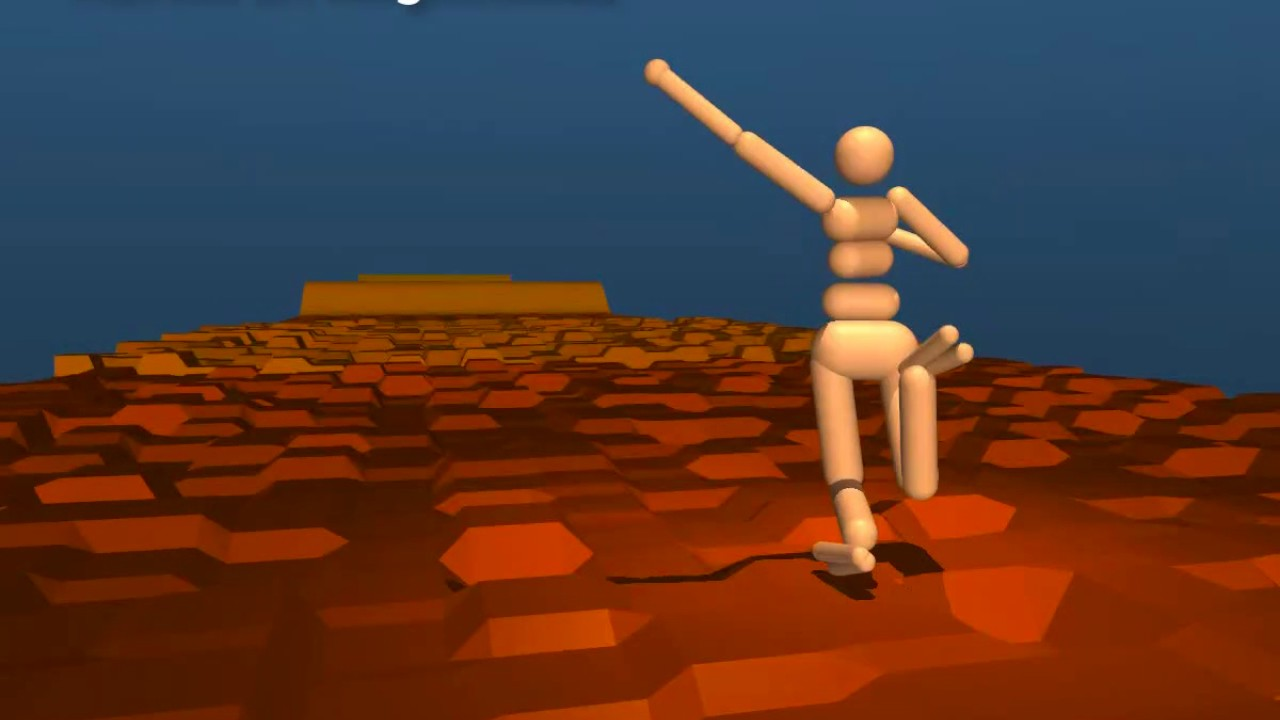
\includegraphics[width=\textwidth]{images/parkour.jpg}
\caption{Robotics~\citep{heess2017emergence}}
\end{figure}
\end{minipage}
\hfill%
\begin{minipage}[t]{.4\paperwidth}
\begin{figure}
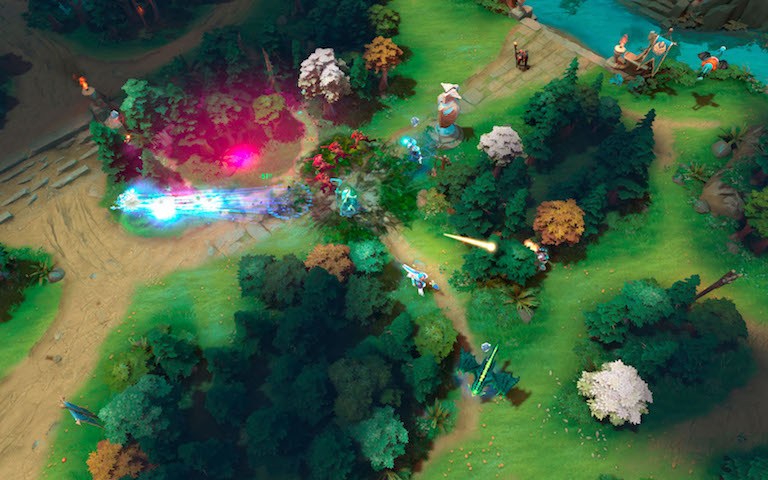
\includegraphics[width=\textwidth, height=3.6cm]{images/dota.jpg}
\caption{Video games~\citep{openaifive}}
\end{figure}	
\end{minipage}

\vspace*{.3cm}

\large{Mostly based on \enb{Stochastic Gradient Ascent}~\citep{robbins1951stochastic}}

\begin{equation*}
\text{maximize } J(\vtheta) \text{ by iterating } \vtheta \gets \vtheta + \alpha \widehat{\nabla}J(\vtheta)
\end{equation*}

\end{frame}

\begin{frame} 
\frametitle{Full vs Stochastic Gradient}
\framesubtitle{Non-convex optimization}
\begin{center}
	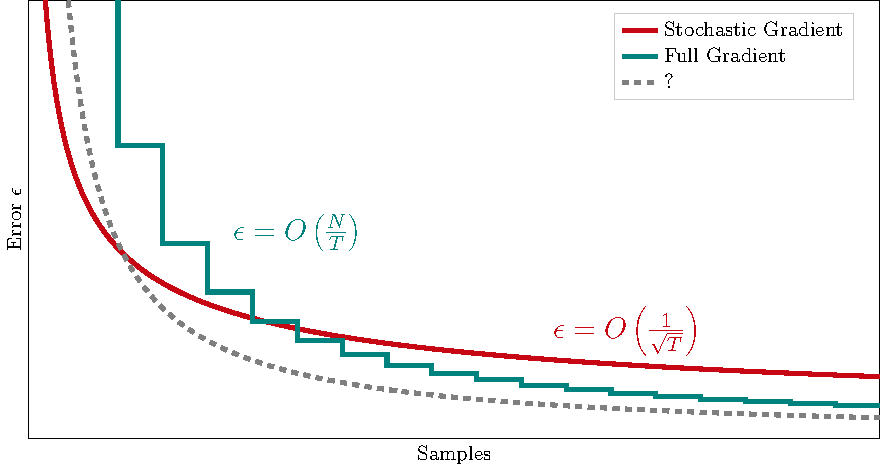
\includegraphics[width=.75\paperwidth]{convergence.pdf}
\end{center}

\vspace*{-.3cm}
\Large{\enb{Can we do something better?}}
\hfill
\small{
Visualization idea from \cite{bachstochastic}
}
\end{frame}

\begin{frame} 
\frametitle{SVRG~\citep{johnson2013accelerating}} 
\framesubtitle{Stochastic Variance-Reduced Gradient}
A solution from \enb{finite-sum optimization}:
\begin{equation*}
	\max_{\vtheta} J(\vtheta) = \sum_{i=1}^{N}f_i(\vtheta)
\end{equation*}
\begin{equation*}
\Large{
	\textcolor{poliblue3}{\underbrace{\blacktriangledown J(\vtheta)}_{\text{SVRG estimator}}}
	= 
	\tikz[baseline]{
		\node[anchor=base, fill=black!4!white, inner sep=10pt]{$
			\textcolor{greenp}{\underbrace{\nabla J(\widetilde{\vtheta}) }_{\text{FG (\textit{snapshot})}}}
			+ 
			\tikz[baseline]{
				\node[anchor=base, fill=black!8!white, inner sep=20pt]{$
					\textcolor{redp}{\underbrace{\nabla f_i(\vtheta)}_{\text{SG in current parameter}}}
					- \textcolor{yellowp}{\underbrace{\nabla f_i(\widetilde{\vtheta})}_{\text{Correction term}}}
					$};
				\node[xshift=-3cm,yshift=.75cm]{\small{\textcolor{black!60}{iteration}}};
			}
			$};
		\node[xshift=-5cm,yshift=1.25cm]{\small{\textcolor{black!40}{epoch}}};
	}	
}
\end{equation*}

\begin{multicols}{2}
\begin{itemize}
	\item Unbiased
	\item Linear convergence
	\item More data-efficient than FG
	\item \enb{Supervised Learning (SL)}
\end{itemize}
\end{multicols}
\end{frame}

\begin{frame} 
\frametitle{SVRG for Reinforcement Learning}
In \enb{Reinforcement Learing (RL)} we maximize \textit{expected return}:

\begin{equation*}
\max_{\vtheta} J(\vtheta) = \int p(\tau\vert\vtheta)R(\tau)d \tau\qquad\text{\citep{peters2008reinforcement}}
\end{equation*}

\vfill

SVRG for RL so far:
\vspace*{.4cm}
\begin{itemize}
	\item \cite{du2017svrgpe} apply SVRG to \textbf{policy evaluation}
	\vspace*{.2cm}
	\item \cite{xu2017svrgtrpo} apply SVRG to \textbf{off-line control}	
\end{itemize}

\vfill

Our work: \enb{on-policy control}
\end{frame}

\begin{frame} 
\frametitle{SVRG for On-Policy Control}
Nontrivial! There are three \eno{challenges}:

\vspace*{.5cm}

\begin{enumerate}
	\item \eno{Non-concavity} of $J(\vtheta)$
		\citep{allen2016variance,reddi2016stochastic}
\vspace*{.5cm}
	\item \eno{Infinite dataset}: we would need \textit{infinite samples} to compute FG~\citep{harikandeh2015stopwasting,bietti2017stochastic}
	\vspace*{.3cm}
	\item \eno{Non-stationarity}: $\tau\sim p_{\textcolor{orange}\vtheta}$ (new!)
\end{enumerate}
\end{frame}

\begin{frame} 
\frametitle{SVRPG} 
\framesubtitle{Stochastic Variance-Reduced \textbf{Policy} Gradient}

\begin{equation*}
\Large{
	\textcolor{poliblue3}{\underbrace{\blacktriangledown J(\vtheta)}_{\text{SVRPG estimator}}}
	= 
	\tikz[baseline]{
	\node[anchor=base, fill=black!4!white, inner sep=15pt]{$
	\textcolor{greenp}{\underbrace{\widehat{\nabla}_N J(\widetilde{\vtheta}) }_{\text{\shortstack{Large N\\to approximate FG}}}}
	+ 
	\tikz[baseline]{
		\node[anchor=base, fill=black!8!white, inner sep=20pt]{$
		\textcolor{redp}{\underbrace{\widehat{\nabla}_B J(\vtheta)}_{B \ll N}}
		- \textcolor{yellowp}{\underbrace{\omega(\vtheta,\widetilde{\vtheta})\widehat{\nabla}_B J(\widetilde{\vtheta})}_{\text{\shortstack{Importance weighting\\for non-stationarity}}}}
		$};
		\node[xshift=-2.5cm,yshift=.75cm]{\small{\textcolor{black!60}{iteration}}};
	}
	$};
	\node[xshift=-5cm,yshift=1.75cm]{\small{\textcolor{black!40}{epoch}}};
	}
	}
\end{equation*}

\begin{itemize}
	\item Unbiased
	\item More data-efficient than FG
	\item \enb{On-policy}: only the correction term is weighted
\end{itemize}

\end{frame}

\begin{frame} 
\frametitle{Convergence Properties} 
Convergence to \eno{local} optimum:

\Large{
\begin{equation*}
	\EVV[]
	{\norm[]{\nabla J(\vtheta)}^2} 
	\leq
	\frac{J(\vtheta^*)-J(\vtheta_0)}{\psi T} +
	\textcolor{orange}{\underbrace{\frac{\zeta}{\mathbf{N}}}_{\text{Infinite dataset}}}
	+\textcolor{orange}{\underbrace{\frac{\xi}{\mathbf{B}}}_{\text{Nonstationarity}}}
\end{equation*}
}

\begin{itemize}
	\item Linear convergence $+$ \eno{error}~\citep [similar to][]{harikandeh2015stopwasting}
	\item $\psi,\zeta,\xi$ depend only on \enb{step size} and \enb{epoch size}
\end{itemize}

\end{frame}

\begin{frame} 
\frametitle{Heuristics} 
Meta-parameter selection

\begin{itemize}
	\item \enb{Adaptive step size}: two ADAM~\citep{kingma2014adam} annealing schedules
	 \begin{equation*}
	 	\underbrace{\alpha_{FG}}_{\text{used at the snapshot}} \qquad \underbrace{\alpha_{SG}}_{\text{used inside epoch}}
	 \end{equation*}
	 \vspace*{.5cm}
	\item \enb{Adaptive epoch size}: new snapshot when effective step size becomes too small
	\begin{equation*}
		\frac{\alpha_{SG}}{B} < \frac{\alpha_{FG}}{N} \implies \textbf{snapshot}
	\end{equation*}
\end{itemize}

\end{frame}

\begin{frame} 
\frametitle{Results} 

%\begin{tikzpicture}

\begin{minipage}[]{.28\paperwidth}
\begin{center}
	\textbf{Cart-Pole}
\end{center}
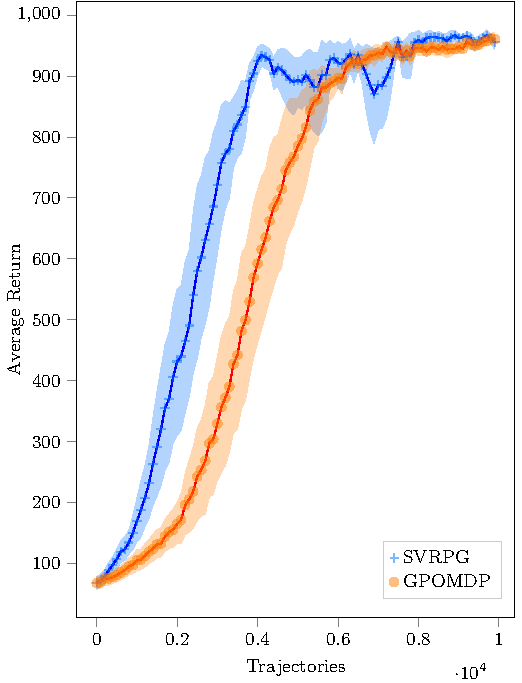
\includegraphics[width=\textwidth]{images/cartpole.pdf}
\end{minipage}
%
\begin{minipage}[]{.28\paperwidth}
\begin{center}
	\textbf{Swimmer}
\end{center}
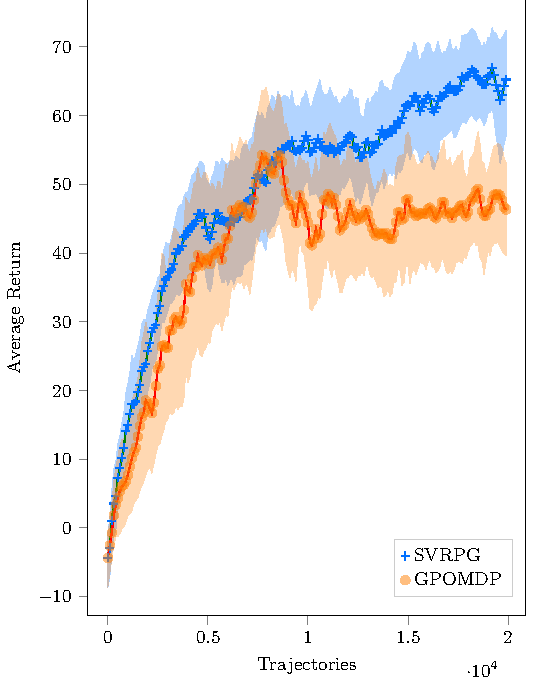
\includegraphics[width=\textwidth]{images/swimmer.pdf}
\end{minipage}
%
\begin{minipage}[]{.28\paperwidth}
\begin{center}
	\textbf{Half-Cheetah}
\end{center}
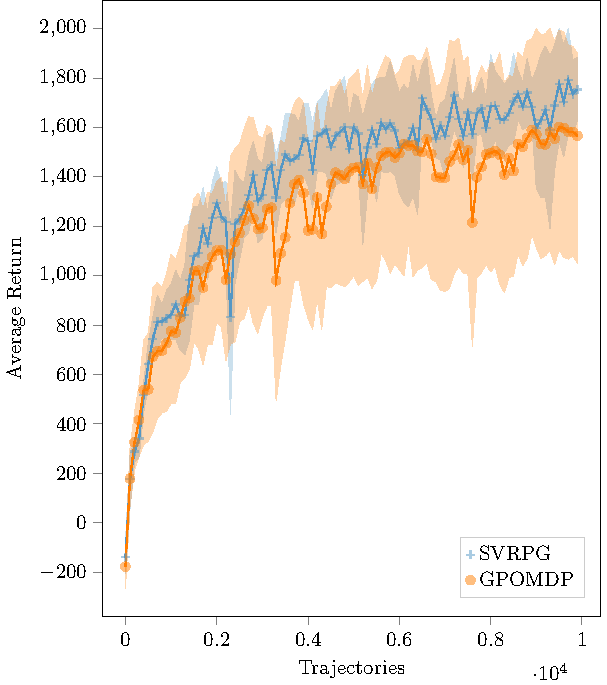
\includegraphics[width=\textwidth]{images/cheetah.pdf}
\end{minipage}

\vfill
\small{
SVRPG: $N=100, B=10$, ADAM 

GPOMDP: $N=10$, ADAM 

Tasks from \textit{rllab}~\citep{duan2016benchmarking}
}
\end{frame}

\begin{frame} 
\frametitle{Conclusions} 

\begin{itemize}
	\item Efficient policy optimization is challenging
	\item \enb{SVRPG}: on-policy control based on SVRG
	\item Meta-parameters still crucial to tame different sources of variance
	\item Future work: adaptive batch size, natural gradient, actor-critic
\end{itemize}

\end{frame}


\begin{frame} 
\frametitle{Thank You} 
\begin{center}
	\Large{\enb{Thank you for your attention}}
\end{center}

\begin{minipage}[]{.6\paperwidth}
\begin{itemize}
	\item Poster: today 06:15 -- 09:00 PM @ \enb{Hall B \#65} 
	\item Contact: \texttt{matteo.papini@polimi.it}
	\item Online resources: \texttt{t3p.github.io}
	\end{itemize}
\end{minipage}
\hfill%
\begin{minipage}[]{.2\paperwidth}

\includegraphics[width=.2\paperwidth]{../qrcode.pdf}
\end{minipage}

\end{frame}


%%%%%%%%%%%%%%%%%%%%%%%%%%%%%%%%%%%%%%%%%%%%%%%%%%%%%%%%%%%%%%%%%%%%%%%%%%%%%%%%%%%%%%%%%
\begin{frame}[allowframebreaks,fragile]
\frametitle{References}
\bibliography{talk.bib}
\end{frame}
%%%%%%%%%%%%%%%%%%%%%%%%%%%%%%%%%%%%%%%%%%%%%%%%%%%%%%%%%%%%%%%%%%%%%%%%%%%%%%%%%%%%%%%%%

%%Backup Slides

\begin{frame} 
\frametitle{SVRPG} 
\framesubtitle{Pseudo-code}

\textbf{For} $s = 1,\ldots$
\vspace*{-.2cm}
\begin{rightbrace2}
	Sample $N$ trajectories using $\widetilde{\theta}$\\
	Compute FG $=\widehat{\nabla}_N J(\widetilde{\theta})$\\
	\textbf{For} $t = 1, \ldots, m$
	\vspace*{-.15cm}
	\begin{rightbrace1}
		Sample $B$ trajectories using $\theta$\\
		Compute SG $=\widehat{\nabla}_B J(\theta)$\\
		Compute correction $=\omega(\theta, \widetilde{\theta})\widehat{\nabla}_B J(\widetilde{\theta})$\\
		Update $\theta\gets\theta+\alpha\gradBlack{\theta}$
	\end{rightbrace1}
	\vspace*{-.15cm}
	Update $\widetilde{\theta}\gets\theta$
\end{rightbrace2}
\vspace*{-.2cm}

\end{frame}

\begin{frame} 
\frametitle{Adaptive Step Size} 
ADAM~\citep{kingma2014adam}:
\begin{itemize}
	\item adapts to gradient variance
	\item can manage different batch sizes
	\item \eno{has memory of past gradients (momentum)}
\end{itemize}
\vfill

\eno{Problem:} FG and SG have very different variance magnitudes \\
$\quad\implies$ spurious momentum
\vfill

We use two \textit{separate} annealing schedules:
\begin{align*}
&\widetilde{\vtheta} \gets \widetilde{\vtheta} + \alpha_{FG}\widehat{\nabla}_NJ(\widetilde{\vtheta})\quad\text{at the snapshot}\\ 
&\vtheta \gets \vtheta + \alpha_{SG}\gradBlack{\vtheta}\quad\text{otherwise}
\end{align*}
\vfill

Note that $\widehat{\nabla}_NJ(\widetilde{\vtheta})\equiv\gradBlack{\vtheta}$ at the snapshot

\end{frame}

\begin{frame} 
\frametitle{Adaptive Epoch Size} 
Epoch size $(m)$ trade-off:
\begin{itemize}
	\item Large $m$ $\implies$ large importance-weighting variance $\implies$ unstable
	\item Small $m$ $\implies$ frequent snapshots $\implies$ data-inefficient
\end{itemize}
\vfill

Idea: ADAM already relates gradient variance and efficiency\\
\vfill

Our stopping criterion:
\begin{equation*}
\frac{\alpha_{SG}}{B} < \frac{\alpha_{FG}}{N} \implies \textbf{snapshot}
\end{equation*}
\vfill

When going on is not \textit{convenient}, take new snapshot
\end{frame}

\begin{frame} 
\frametitle{Normalized Importance Weighting} 

\begin{minipage}[]{.45\paperwidth}
Regular importance weighting (unbiased):
\begin{equation*}
	\omega(\vtheta,\widetilde{\vtheta})\widehat{\nabla}_B J(\widetilde{\vtheta}) = \frac{1}{B}\sum_{i=1}^B\frac{p(\tau_i\vert\widetilde{\vtheta})}{p(\tau_i\vert\vtheta)}\nabla\log p(\tau_i\vert\widetilde{\vtheta})R(\tau_i)
\end{equation*}
\vfill

Normalized importance weighting:
\begin{equation*}
\omega(\vtheta,\widetilde{\vtheta})\widehat{\nabla}_B J(\widetilde{\vtheta}) = \frac{\sum_{i=1}^B\frac{p(\tau_i\vert\widetilde{\vtheta})}{p(\tau_i\vert\vtheta)}\nabla\log p(\tau_i\vert\widetilde{\vtheta})R(\tau_i)}
	{\sum_{i=1}^B\frac{p(\tau_i\vert\widetilde{\vtheta})}{p(\tau_i\vert\vtheta)}}
\end{equation*}
\vfill

\begin{itemize}
	\item Less variance at the price of small bias
	\item Only affects the correction term
	\item Benefits are task-dependent
\end{itemize}
\end{minipage}
\hfill%
\begin{minipage}[]{.35\paperwidth}
	\begin{center}
		\textbf{Swimmer}
	\end{center}
	\vspace*{-.25cm}
	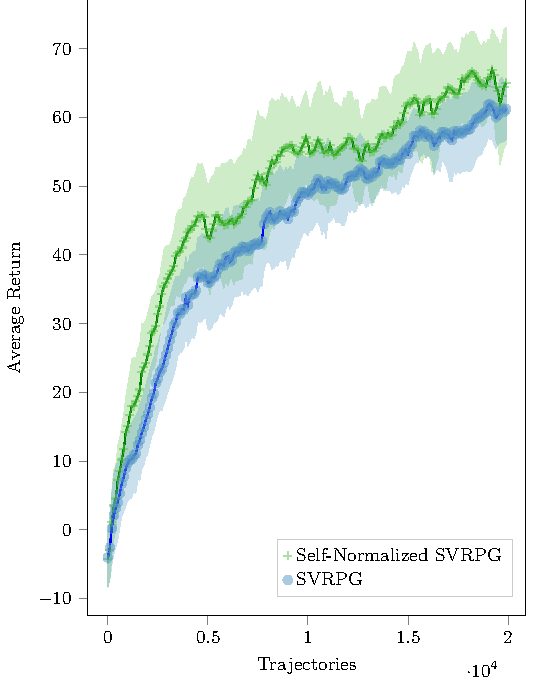
\includegraphics[width=\textwidth]{images/normalization.pdf}
\end{minipage}

\end{frame}

\begin{frame} 
\frametitle{Actor-Critic SVRPG}
\framesubtitle{Preliminary results}

\enb{Critic} (or \textit{baseline}): an orthogonal variance-reduction technique
\begin{equation*}
	\text{Gradient sample: } \sum_{t=1}^{H}\left(\sum_{k=1}^t\nabla\log\pi_{\vtheta}(a_t\vert s_t)\right)(\gamma^tr_t - \underbrace{\mathbf{b}}_{\text{baseline}})\quad\text{\citep{peters2008reinforcement}}
\end{equation*}
\vfill
\eno{Not trivial} to combine SVRG with critic: variance reduction is not additive\\
\vfill
We combine SVRG with a simple critic from~\citet{duan2016benchmarking}\\
\vfill
Future work: ad hoc critic

\end{frame}

\begin{frame} 
\frametitle{The Full Story} 

\begin{minipage}[]{.45\paperwidth}
	\begin{itemize}
		\item For \textbf{Swimmer}, we employ normalized weights in our final result
		\item For \textbf{Half-Cheetah}, we employ normaized weights \textit{and} critic in our final result
		\item We compare \enb{SVRPG} with GPOMDP~\citep{baxter2001infinite} with batch size $B = 10$
		\item This shows the \textit{advantage} of 	correcting SG with more data
		\item However, GPOMDP with batch~size~$N = 100$ is even worse
	\end{itemize}
\end{minipage}
\hfill%
\begin{minipage}[]{.35\paperwidth}
	\begin{center}
	\textbf{Half-Cheetah}
\end{center}
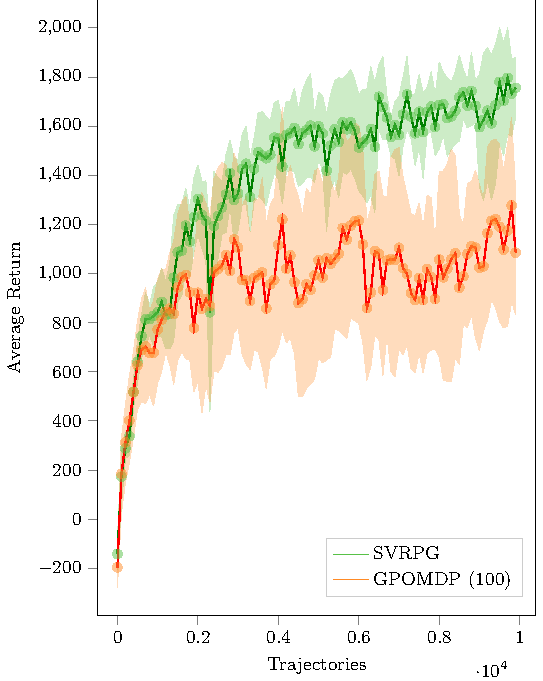
\includegraphics[width=.9\textwidth]{images/cheetah100.pdf}
\end{minipage}

\end{frame}

\end{document}